\subsection{排序}
\begin{formal}
    {\cuhei 问题描述:}

    排序算法分为简单排序(时间复杂度为$O(n^2)$)和高效排序(时间复杂度为$O(n\log n)$)。

    请自行随机生成不同规模的数据(例如10,100,1K,10K,100K,1M,10K正序,10K逆序),用不同的排序算法(快速排序,归并排序,堆排序,选择排序,冒泡排序,直接插入排序,希尔排序)
    分别对这些数据进行测试,输出运行时间,并总结各种排序算法的特点、时间复杂度、空间复杂度,以及是否是稳定排序和部分排序。
\end{formal}
\begin{formal}
    {\cuhei 输入要求:}

    第1行一个正整数$n$,表示元素个数。第2行$n$个整数,用空格分割。$1\leq n\leq 100000$
\end{formal}
\begin{formal}
    {\cuhei 输出要求:}

从小到大排序后的结果,以空格分割。
\end{formal}
\subsubsection{数据结构设计}
\begin{lstlisting}[name=Q1]
vector<int> nums;
vector<int> gaps;//用于希尔排序
\end{lstlisting}
\subsubsection{功能描述}
\begin{function}
    \tcp*[h]{$a_0$为公差为gap的子序列的第一个元素。当 $a_0=1,gap=1$时,便是直接插入排序}\;
    \SetKw{by}{by}
    \SetKwFunction{Swap}{Swap}
    \For{i=$a_0+gap$ \KwTo nums.length \by gap}
    {
        j = i-gap\;
        key = nums[i]\;
        \While{j $\geq a_0$ and nums[j]>key}
        {
        nums[j+gap]=nums[j]\;
        j = j-gap\;
        }
        nums[j+gap]=key\;
    }
    \caption{Insert-Sort-with-Gap(nums,$a_0$,gap)}
\end{function}
\begin{algorithm}[H]
    \SetKwFunction{Select}{Select-Sort-with-Gap}
    \SetKw{in}{in}
    \ForEach{gap \in gaps}
    {
        \lFor{i = 0 \KwTo gap-1}{\Select(nums,i,gap)}
    }
    \caption{Shell-Sort(nums,gaps)}
\end{algorithm}
\begin{algorithm}
    \SetKwFunction{Swap}{Swap}
    \SetKw{break}{break}
    \For{i = 1 \KwTo nums.length-1}
    {
        change = 0
        \For{j = 1 \KwTo nums.length-1}
        {
            \lIf{nums[j+1]<nums[j]}{\Swap(nums[j],nums[j+1])}    
            change = 1\;
        }
        \lIf{change == 0}{\break}
    }
    \caption{Bubble-Sort(nums)}
\end{algorithm}
\begin{algorithm}
    \For{i = 1 \KwTo nums.length-1}
    {
        min = i\;
        \For{j = i+1 \KwTo nums.length}
        {
            \lIf{nums[j]<nums[min]}{min = j}
        }
        \lIf{min $\neq$ i}{\Swap(nums[min],nums[i])}
    } 
    \caption{Select-Sort(nums)}
\end{algorithm}
\subsubsection{调试分析}
最初测试归并排序和快速排序时,发现均有5个样例出现超时的现象,不符合预期。经过排查后也没有发现逻辑上的问题,
最终发现是因为递归函数的返回值是一整个vector,但是并没有以引用的形式返回,导致需要大量额外的内存拷贝。将返回变量改为引用形式后,
测试结果便正常了。

\subsubsection{总结和体会}
使用希尔排序时,当gaps设置为5,3,1和4,2,1时,样例7均无法通过;当设置为8,4,2,1时,能通过所有样例。

使用插入排序时,无法通过样例5,7,9 。

使用冒泡排序时,当使用change变量判断排序是否完成时,无法通过样例5,7,8,9 ;不使用时,则无法通过样例5,6,7,8,9 。

使用选择排序时,无法通过样例5,6,7,8,9.

使用归并排序和堆排序时,可以通过所有样例。

使用以末端元素作为枢纽的快速排序时,无法通过样例6,7,8.

由此可以推断出:
\begin{itemize}
    \item 样例7逆序对较多 
    \item 样例6的原始序列大部分已经排序完成
    \item 样例5,6,7,8,9待排序元素较多
    \item 样例6,7,8数据的分布会使得快速排序退化。
\end{itemize}
\begin{figure}
    \centering
    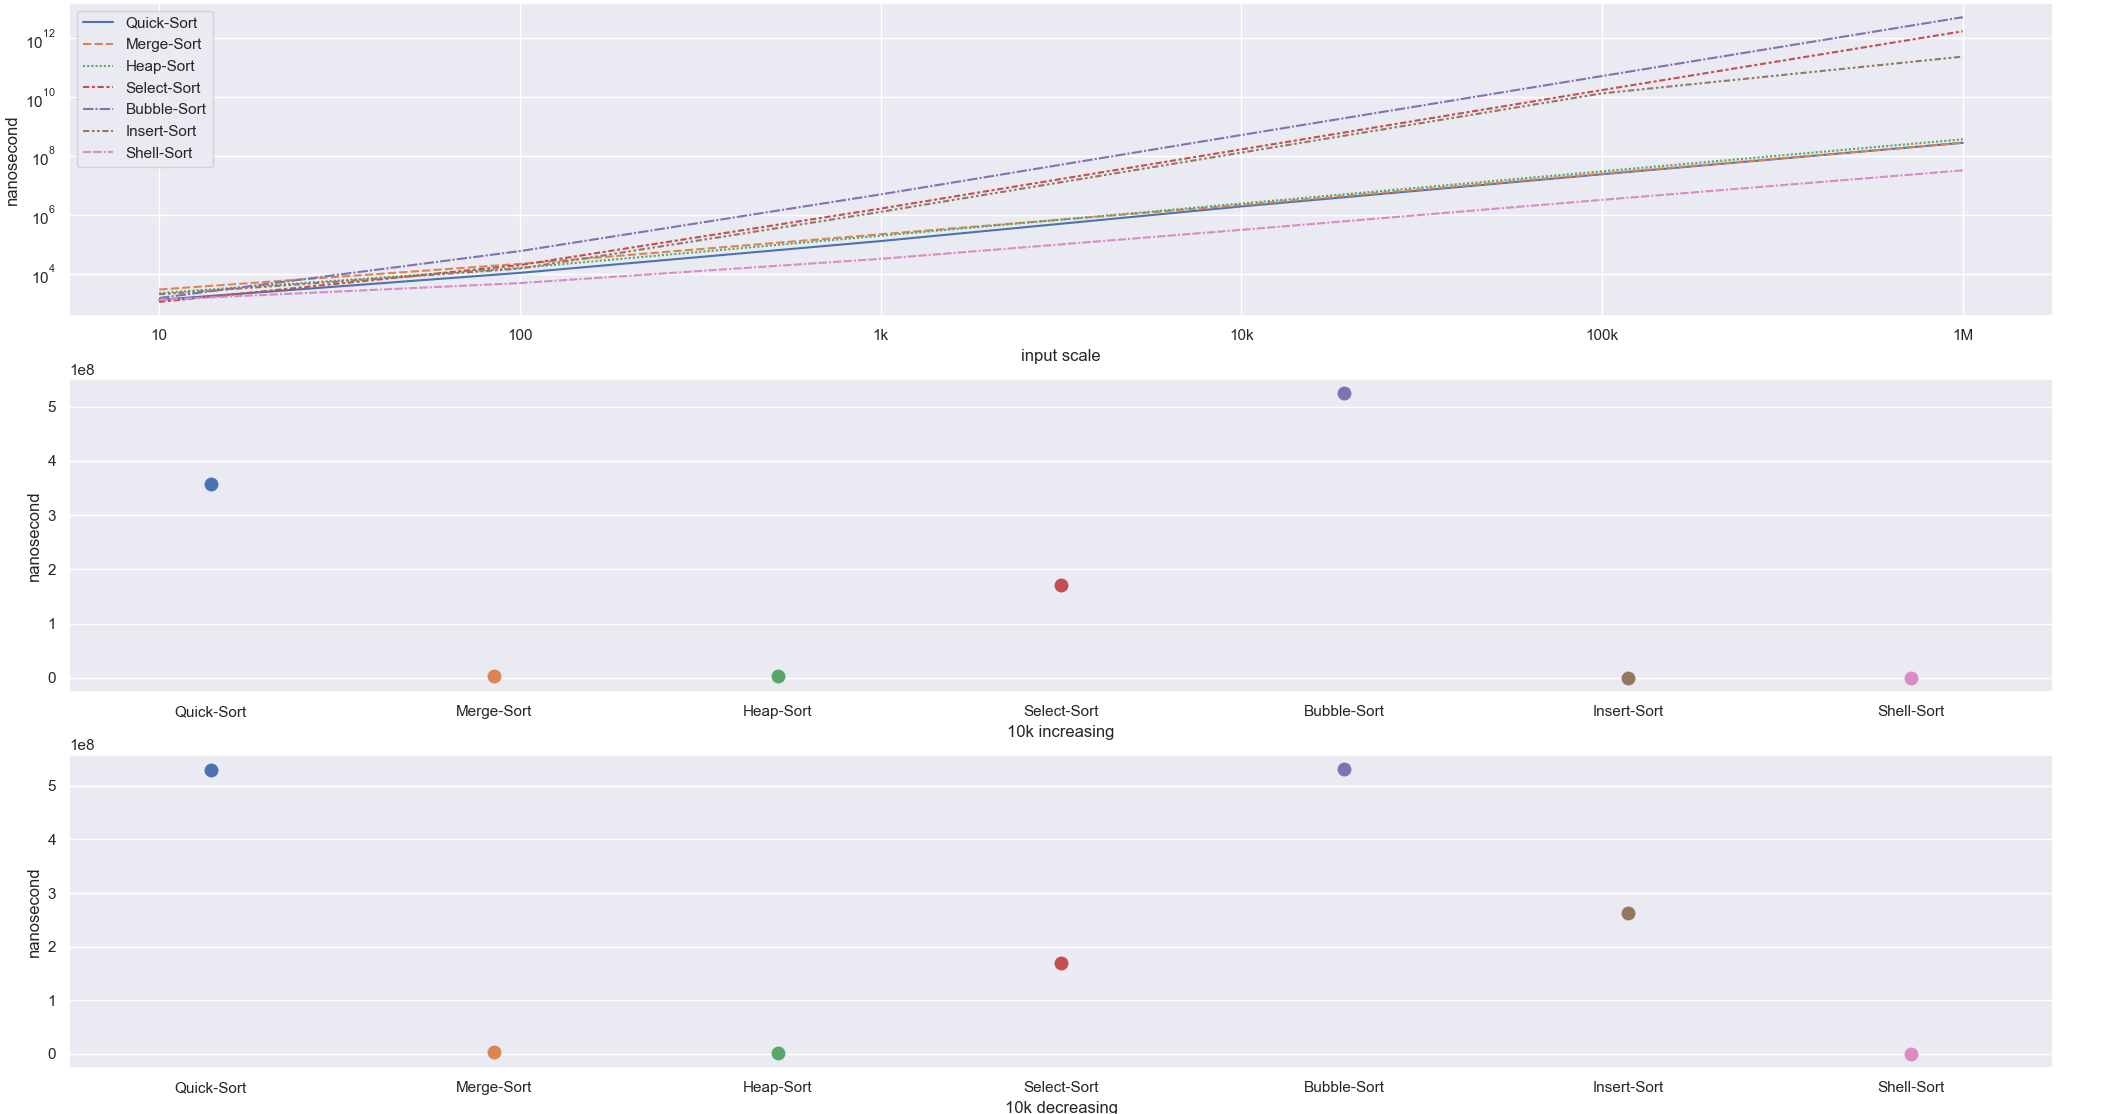
\includegraphics[width=\textwidth]{fig1.png}
    \caption{各算法运行时间}
\end{figure}
\begin{table}
\centering    
\begin{tabular}[h]{r|r|r|r|r|r|r}
      nanosecond  & 10   &  100   &   1k    &    10k    &   100k   &   1M   \\\hline
Quick-Sort& 1300& 10700& 129000& 1939500& 24167500& 283930100\\\hline
Merge-Sort& 2900& 21600& 219600& 2172600& 25443000& 283943100 \\\hline
Heap-Sort& 2200& 15800& 195800& 2443000& 30363500& 372333700 \\\hline
Select-Sort& 1100& 19700& 1641100& 168638300& 17555834200& 1754645573400 \\\hline
Bubble-Sort& 1500& 58800& 4971400& 520298700& 52657170700& 5270084636700 \\\hline
Insert-Sort& 2000& 15000& 1268000& 131088000& 13537059000& 240677606000 \\\hline
Shell-Sort& 1300& 4800& 32100& 310000& 3250400& 32636200 
\end{tabular}
\begin{tabular}[h]{r|r|r}
      nanosecond  &10k increaing&10k decreasing  \\\hline
Quick-Sort& 356991600& 529755200 \\\hline
Merge-Sort&  2764800& 3034900 \\\hline
Heap-Sort&  2458500& 2496800 \\\hline
Select-Sort&  170450800& 168860200 \\\hline
Bubble-Sort&  525029500& 531327100 \\\hline
Insert-Sort&  91000& 263311000 \\\hline
Shell-Sort&  317800& 612800 
\end{tabular}
\caption{各算法运行时间}
\end{table}
\begin{table}
\centering    
\begin{tabular}[h]{r|c|c|c|c|c}
       &比较次数&移动次数&附加存储空间&稳定排序&部分排序\\
\hline 快速排序&   $\Omega(n\lg n),O(n^2)$   &  $\Omega(n\lg n),O(n^2)$ &    $\Omega(\lg n),O(n)$     &   $\times$     &   $\times$  \\
\hline 归并排序&   $\Theta(n\lg n)$   & $\Theta(n\lg n)$  &    $\Theta(n)$     &    $\surd$    &   $\times$   \\
\hline 堆排序&    $\Theta(n\lg n)$   & $\Theta(n\lg n)$ &     $\Theta(1)$    &     $\times$   &    $\surd$  \\
\hline 选择排序&    $\Theta(n^2)$  & $O(n)$  &    $\Theta(1)$     &    $\times$    &   $\surd$   \\
\hline 冒泡排序&   $\Omega(n),O(n^2)$    & $O(n^2)$ &    $\Theta(1)$     &     $\surd$   &   $\surd$   \\
\hline 直接插入排序&  $\Omega(n),O(n^2)$  & $O(n^2)$    &   $\Theta(1)$      &   $\surd$     &    $\times$  \\
\hline 希尔排序&   $\Omega(n),O(n^2)$   &  $O(n^2)$  &   $\Theta(1)$      &     $\times$   &    $\times$  \\
\end{tabular}
\caption{各算法特点总结}
\end{table}
\begin{itemize}
    \item 快速排序:是高效排序,并且平均而言性能更加突出,但是遇到某些输入时会退化为简单排序。同时由于是采用递归实现,会占用一定的空间
    \item 归并排序:是高效排序,且性能不受输入数据的初始状态影响,具有稳定性,但是需要较多的附加存储空间
    \item 堆排序:是高效排序,且性能不受输入数据的初始状态影响,且具有部分排序功能
    \item 选择排序:直观易懂,具有部分排序功能,性能较差,但是移动次数较少
    \item 冒泡排序:直观易懂,具有稳定性,部分排序功能,但性能较差
    \item 直接插入排序:直观易懂,具有稳定性,但性能较差
    \item 希尔排序:性能受gap的取值影响较大
\end{itemize}